% CAST pipeline figure (Fig. 1). Rendered natively with TikZ, single column.
% Supporting macros, colors, and the PDDL listings language live in main.tex.
\begin{figure}[t]
  \centering
  % --- captured PDDL code panels ---
  \begin{lrbox}{\pddlDomA}\begin{lstlisting}[style=pddl]
(define (domain stretch_cleanup)
  (:requirements :strips :typing)
  (:types robot graspable - object
          eraser - graspable
          whiteboard - object)
  { ... })
\end{lstlisting}\end{lrbox}%
  \begin{lrbox}{\pddlProbU}\begin{lstlisting}[style=pddl]
(define (problem stretch_cleanup_0)
  (:domain stretch_cleanup)
  (:objects
    stretch      - object
    cloth_0      - object
    whiteboard_0 - object
    marker_0     - object
    mug_0        - object)
  (:goal (whiteboard_clean whiteboard_0)))
\end{lstlisting}\end{lrbox}%
  \begin{lrbox}{\pddlProbT}\begin{lstlisting}[style=pddltyped]
(define (problem stretch_cleanup_0)
  (:domain stretch_cleanup)
  (:objects
    stretch      - robot
    cloth_0      - graspable
    whiteboard_0 - whiteboard
    marker_0     - graspable
    mug_0        - graspable)
  (:goal (whiteboard_clean whiteboard_0)))
\end{lstlisting}\end{lrbox}%
  % equalize all panel widths to the widest (the problem panels)
  \setlength{\panelw}{\wd\pddlProbU}%
  \ifdim\wd\pddlProbT>\panelw \setlength{\panelw}{\wd\pddlProbT}\fi
  \resizebox{\columnwidth}{!}{%
  \begin{tikzpicture}[
      stage/.style={draw=stagerule,rounded corners=4pt,fill=stagebg,inner sep=5pt},
      bigbox/.style={draw=stagerule,rounded corners=3pt,fill=stagebg,
                     align=center,font=\bfseries,inner sep=5pt,minimum width=3.2cm},
      flow/.style={-{Stealth[length=2.6mm,width=2.6mm]},line width=1pt,accent},
    ]
    % left-column anchor: physical task at origin
    \node[bigbox,anchor=north] (photo) at (0,0)
        {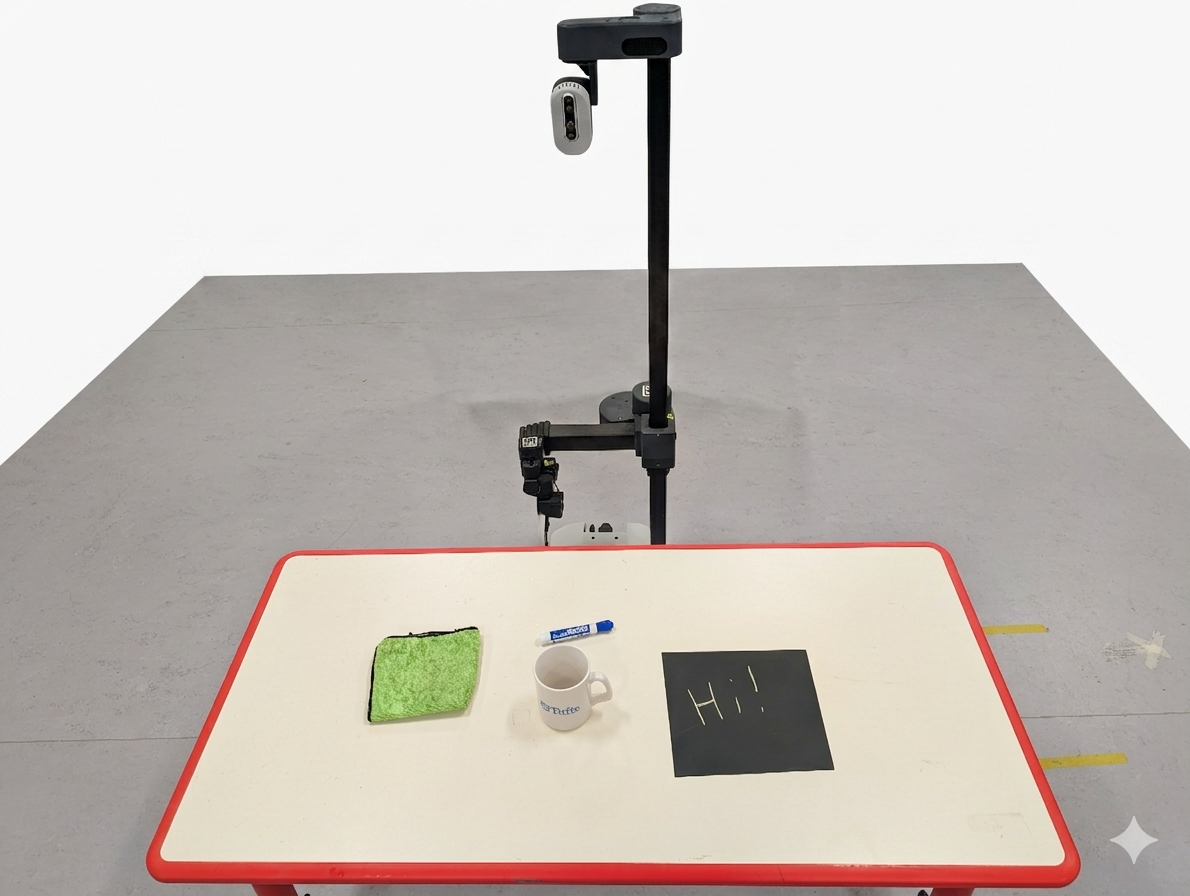
\includegraphics[width=3cm]{figures/robot_photo.png}\\[1pt]Physical Task};

    % right column: the two PDDL stages, placed RELATIVE to the photo
    % (fixed gap) so font-metric differences never cause overlap
    \node[stage,anchor=north west] (rt) at ([xshift=1.1cm]photo.north east) {%
      \begin{tabular}{@{}c@{}}
        {\footnotesize\bfseries\color{accent} Runtime Generated PDDL} {\scriptsize (with Typing Gap)}\\[1pt]
        \pddlpanel{Typed Domain}{\usebox\pddlDomA}\\[1pt]
        \pddlpanel{Untyped Problem}{\usebox\pddlProbU}
      \end{tabular}};
    % The domain is unchanged by the LLM (only the problem's object types are
    % repaired), so it is shown once above; this stage shows just the repaired problem.
    \node[stage,anchor=north,below=0.4cm of rt] (ll) {%
      \begin{tabular}{@{}c@{}}
        {\footnotesize\bfseries\color{accent} LLM Typed PDDL} {\scriptsize (Repaired Problem)}\\[1pt]
        \pddlpanel{Typed Problem}{\usebox\pddlProbT}
      \end{tabular}};

    % left column: remaining actors, spread to match right-column height
    \node[bigbox,anchor=south] (planner) at (photo.south |- ll.south)
        {
\includegraphics[width=1.15cm]{figures/icon_planner.png}\\[1pt]Symbolic Planner};
    \node[bigbox] (llm) at (photo.south |- {$(rt.south)!0.5!(ll.north)$})
        {
\includegraphics[width=1.1cm]{figures/icon_llm.png}\\[1pt]CAST LLM\\Preprocessing};

    % zig-zag flow: photo -> rt -> llm -> ll -> planner -> photo.
    % The LLM's incoming and outgoing arrows both attach at (llm.east) with
    % mirror-image arcs so they read as a single pass-through point.
    \draw[flow] (photo.east) -- (photo.east -| rt.west);
    \draw[flow] (rt.west)  to[out=180,in=0] (llm.east);
    \draw[flow] (llm.east) to[out=0,in=180] (ll.west);
    \draw[flow] (ll.west)  to[out=180,in=0] (planner.east);
    % feedback loop routed around the far left, clear of the LLM box
    \coordinate (FL) at ([xshift=-0.55cm]photo.west);
    \draw[flow] (planner.west) -- (planner.west -| FL)
          -- (photo.west -| FL) -- (photo.west);
  \end{tikzpicture}}
  \caption{\small{The CAST typing pipeline. A physical task is encoded at runtime into a typed domain and a problem whose objects carry only an overly-general base type, leaving the goal unreachable (the typing gap). The LLM reassigns each object a functional type already defined in the domain (highlighted), and the repaired problem is handed to a symbolic planner.}}
    \label{fig:robot_example}
\end{figure}